\documentclass{beamer}

\documentclass{beamer}
\usepackage[utf8]{inputenc}
\usepackage[ngerman]{babel}
\usepackage{url}
\usepackage{xcolor}

\usetheme[compress]{Berlin}
\setbeamerfont{headline}{size=\large}
\setbeamerfont*{section in head/foot}{size=\tiny}
\setbeamertemplate{toc}{circle}
\setbeamertemplate{itemize subitem}[triangle] % if you want a triangle
\setbeamercovered{transparent}

\definecolor{myBlue}{rgb}{0,0.55,0.8}
\usecolortheme[named=myBlue]{structure}

\title{Das \LaTeX-KBS}
\subtitle{\small Grundlagen von \LaTeX, Ti\textit{k}Z und Co.}
\author
{
	Walter Stieben \texttt{\href{mailto:4stieben@informatik.uni-hamburg.de}{4stieben@inf}}\\
	\href{http://hauke-stieler.de/}{Hauke Stieler} \texttt{\href{mailto:4stieler@informatik.uni-hamburg.de}{4stieler@inf}}
}
\date{\footnotesize 12.01.2016}

\begin{document}
	\maketitle
	\tableofcontents\newpage
	\section{Was ist \TeX{} und \LaTeX{}}
		\subsection*{asd}
		\begin{frame}{Was ist \LaTeX{}}
			\textbf{\LaTeX{} und \TeX{}:}
			\begin{itemize}
				\item \TeX{} ist ein Textsatzsystem von Donald E. Knuth
				\item \LaTeX{} ist ein Satz von Makros für \TeX
				\item WYSIWYT (What You See Is What You Type)
			\end{itemize}
			\vspace{0.2cm}
			\textbf{Vorteile von \LaTeX{}:}
			\begin{itemize}
				\item Ergebnis sieht hübsch aus
				\item \LaTeX{} kümmert sich um die Formatierung
				\item Der Quelltext lässt sich Versionsverwalten
				\item Für mathematische Formeln sehr gut
				\item ``Ich möchte X mit \LaTeX{} machen'' $\rightarrow$
				Suchmaschine: ``latex X'' eingeben $\rightarrow$
				Ergebnis in den Quelltext kopieren
			\end{itemize}
		\end{frame}
\end{document}

\title{Das \LaTeX-KBS}
\subtitle{\small Grundlagen von \LaTeX, Beamer und Tipps für Hausaufgaben, Seminararbeiten, etc.}

\date{\footnotesize \today}

\begin{document}
	\maketitle
		
	%%%%%%%%%%%%%%%%%%%%%%%%%%%%%%%%%%%%%%%%%%%%%%%%%%%%%%%%%%%%%%%%%%%%%%%
		
	\begin{frame}
		\begin{center}
			Danke Henning (\texttt{8pridoeh}) dass wir deine Folien aus dem WS14/15 benutzen dürfen :D
		\end{center}
		Und auch Danke an alle, die zu den Folien und zum Vortrag beigetragen haben:
		\begin{itemize}
			\item Walter Stieben \texttt{\href{mailto:4stieben@informatik.uni-hamburg.de}{4stieben@inf}}\\
			\item Ruben Felgenhauer \texttt{\href{mailto:4felgenh@informatik.uni-hamburg.de}{4felgenh@inf}}\\
			\item Malte Hamann \texttt{\href{mailto:1hamann@informatik.uni-hamburg.de}{1hamann@inf}}\\
			\item Hauke Stieler \texttt{\href{mailto:4stieler@informatik.uni-hamburg.de}{4stieler@inf}}
		\end{itemize}
	\end{frame}
		
	%%%%%%%%%%%%%%%%%%%%%%%%%%%%%%%%%%%%%%%%%%%%%%%%%%%%%%%%%%%%%%%%%%%%%%%
		
	\begin{frame}
		\begin{minipage}[0.5\textheight]{0.5\textwidth}
			\tableofcontents[hideallsubsections]
		\end{minipage}
		\begin{minipage}{0.45\textwidth}
			
\includegraphics[width=1.05\textwidth]{./images/gib-word-keine-chance}
		\end{minipage}
	\end{frame}
		
	%%%%%%%%%%%%%%%%%%%%%%%%%%%%%%%%%%%%%%%%%%%%%%%%%%%%%%%%%%%%%%%%%%%%%%%
		
	\section{Was ist \LaTeX{}}
		\subsection{Einführung}
		\begin{frame}{Was ist \LaTeX{}}
			\slideheading{\LaTeX{} und \TeX{}:}
			\begin{itemize}
				\item \TeX{} ist ein Textsatzsystem von Donald E. Knuth
				\item \LaTeX{} ist ein Satz von Makros für \TeX
				\item WYSIWYM (What You See Is What You Mean)
			\end{itemize}
			\vspace{0.1cm}
			\slideheading{Vorteile von \LaTeX{}:}
			\begin{itemize}
				\item Ergebnis sieht hübsch aus
				\item \LaTeX{} kümmert sich um die Formatierung
				\item Der Quelltext lässt sich Versionsverwalten
				\item Für mathematische Formeln sehr gut
				\item ``Ich möchte X mit \LaTeX{} machen'' $\rightarrow$
				Suchmaschine: ``latex X'' eingeben $\rightarrow$
				Ergebnis in den Quelltext kopieren
				\item Der meiste Code ist wiederverwendbar
			\end{itemize}
		\end{frame}
		
		%%%%%%%%%%%%%%%%%%%%%%%%%%%%%%%%%%%%%%%%%%%%%%%%%%%%%%%%%%%%%%%%%%%%%%%
		\subsection{\LaTeX{} installieren}
		\begin{frame}{\LaTeX-Distribution}
%			\slideheading{\LaTeX-Distribution:}
Die \LaTeX-Distribution stellt eine Sammlung von Paketen und Programmen zum Kompilieren bereit (Backend). \\
			\begin{description}
				\item[GNU/Linux] Nutzt den Paketmanager eurer Distribution. Debian/Ubuntu: \texttt{apt-get install texlive} \\
				oder \texttt{apt-get install texlive-full} (\(>\) 2 GB)
				\item[Windows] MiKTeX  oder TeX Live herunterladen und installieren. \url{http://miktex.org/} \url{http://www.tug.org/texlive/}
				\item[Mac OS] MacTex herunterladen und installieren. \url{http://tug.org/mactex/} 
			\end{description}
			\end{frame}	
			
			
		\begin{frame}{\LaTeX-Editoren}
%			\slideheading{\LaTeX-Editoren:}
			\begin{description}
				\item[Kile] Guter Editor für GNU/Linux (KDE).
				\item[Gummi] Editor für GNU/Linux (GTK) mit Live-Preview
				\item[AUCTeX] für Emacs-Benutzer
				\item[Texmaker] Editor für alle Betriebssysteme
				\item[Texstudio] Fork von Texmaker mit mehr Funktionen
			\end{description}
			 und viele mehr \dots
		\end{frame}
		
		%%%%%%%%%%%%%%%%%%%%%%%%%%%%%%%%%%%%%%%%%%%%%%%%%%%%%%%%%%%%%%%%%%%%%%%

% Man muss sich bei Overleaf wohl jetzt registrieren :'(
%		\begin{frame}{Overleaf}
%			Online Editor mit Live-Preview (\url{https://www.overleaf.com})
%			
%			\begin{center}
%				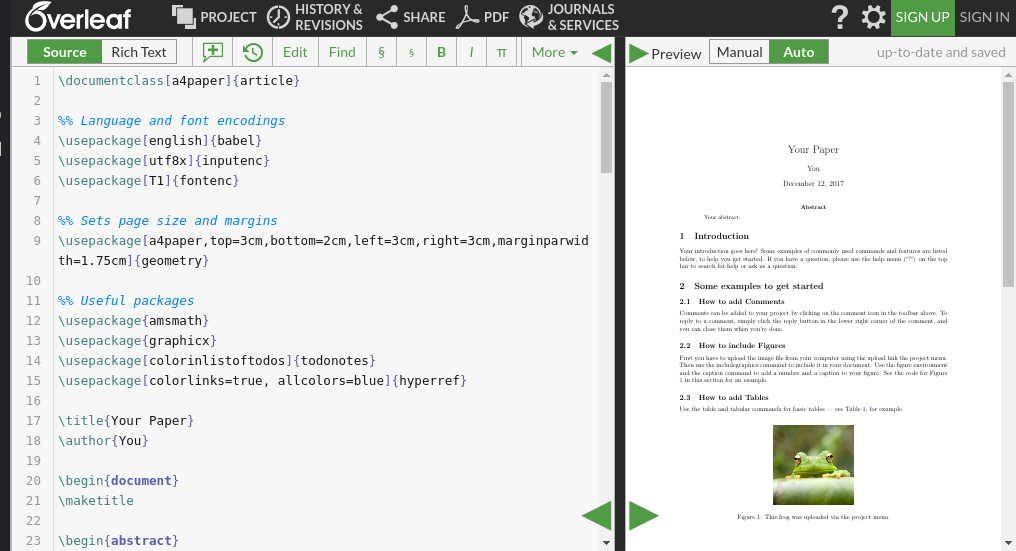
\includegraphics[width=0.75\textwidth]{images/overleaf}
%			\end{center}
%		\end{frame}
		
		%%%%%%%%%%%%%%%%%%%%%%%%%%%%%%%%%%%%%%%%%%%%%%%%%%%%%%%%%%%%%%%%%%%%%%%
		
		\begin{frame}{Latexbase}
			Online Editor mit Live-Preview (\url{https://latexbase.com})
			
			\begin{center}
				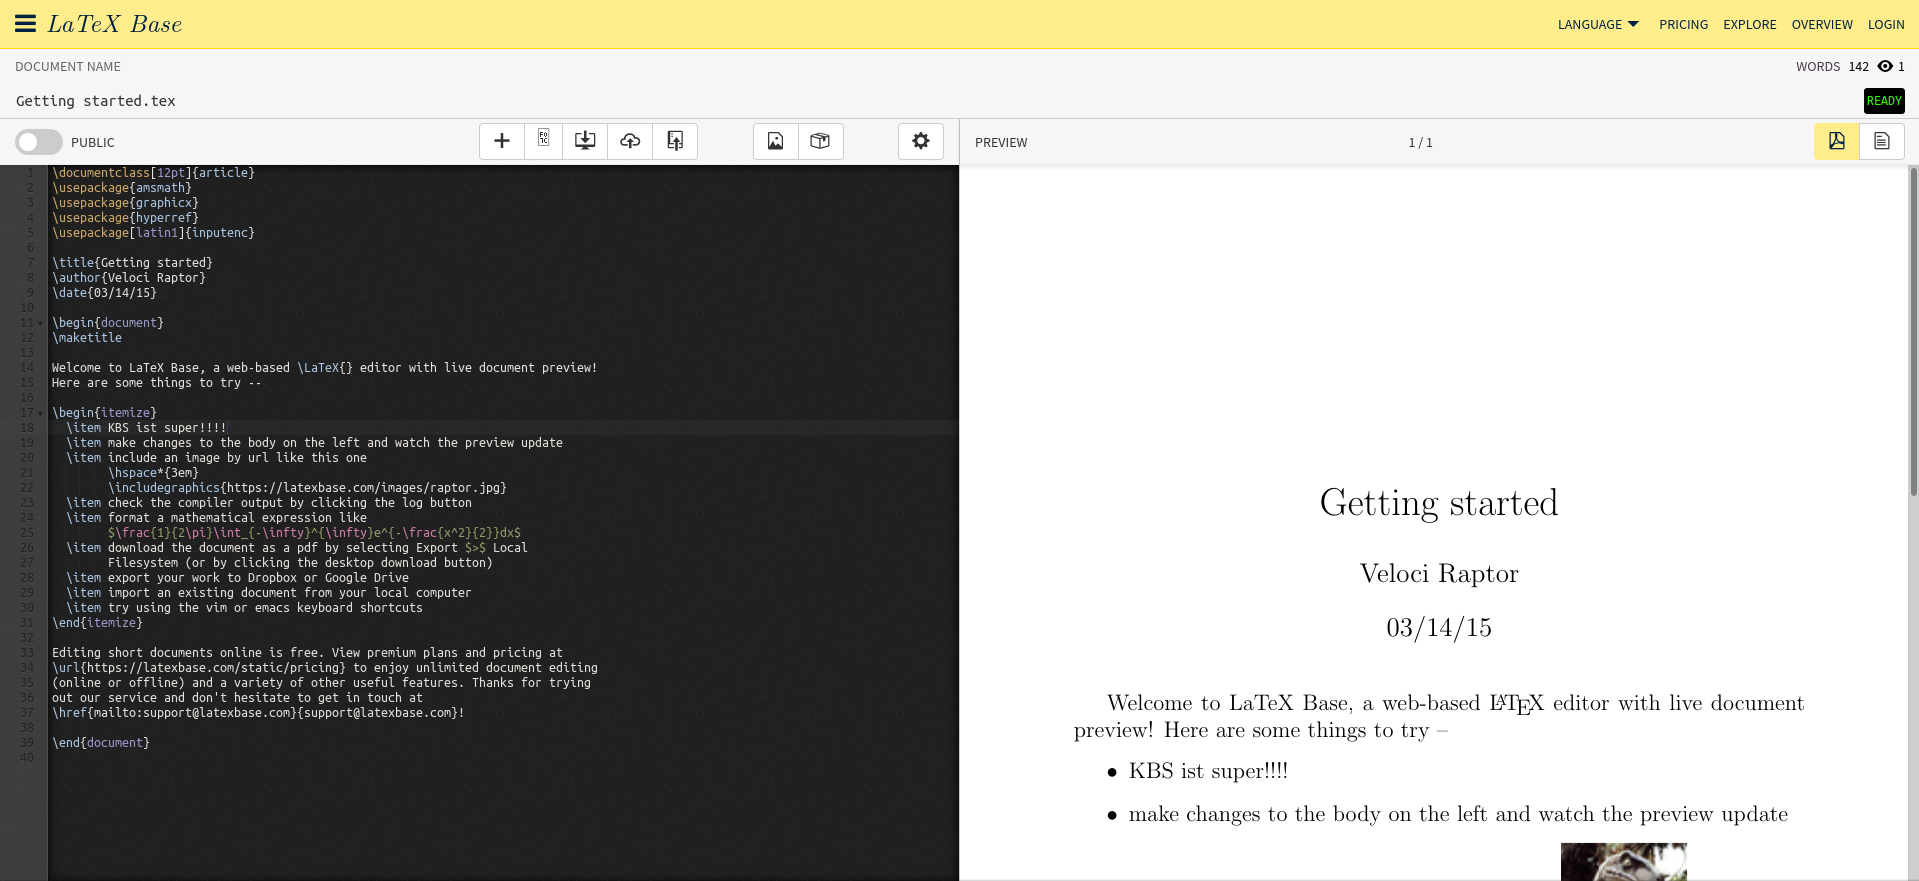
\includegraphics[width=0.85\textwidth]{images/latexbase}
			\end{center}
		\end{frame}
		
		%%%%%%%%%%%%%%%%%%%%%%%%%%%%%%%%%%%%%%%%%%%%%%%%%%%%%%%%%%%%%%%%%%%%%%%
		
		\begin{frame}{Verschiedene \LaTeX{}-Compiler}
			Es gibt verschiedenen Compiler für \LaTeX{}. Heute: \textbf{pdflatex}
			\slideheading{Vorteile von pdflatex:}
			\begin{itemize}
				\item Direktes erzeugen einer PDF
				\item Viele PDF-Features nutzbar
				\item Einfach zu verwenden
			\end{itemize}
			\slideheading{Nachteile von pdflatex:}
			\begin{itemize}
				\item Kein \texttt{pstricks} nutzbar.
				\item Postscript-Dateien nicht direkt einbindbar
				\item Keine vollständige Unicode-Unterstützung (wie Xe\LaTeX)
			\end{itemize}
		\end{frame}
		
		%%%%%%%%%%%%%%%%%%%%%%%%%%%%%%%%%%%%%%%%%%%%%%%%%%%%%%%%%%%%%%%%%%%%%%%
		
		\begin{frame}{Detexify -- \LaTeX-Symbolerkennung}
		\begin{minipage}[0.5\textheight]{0.5\textwidth}
			\begin{center}
			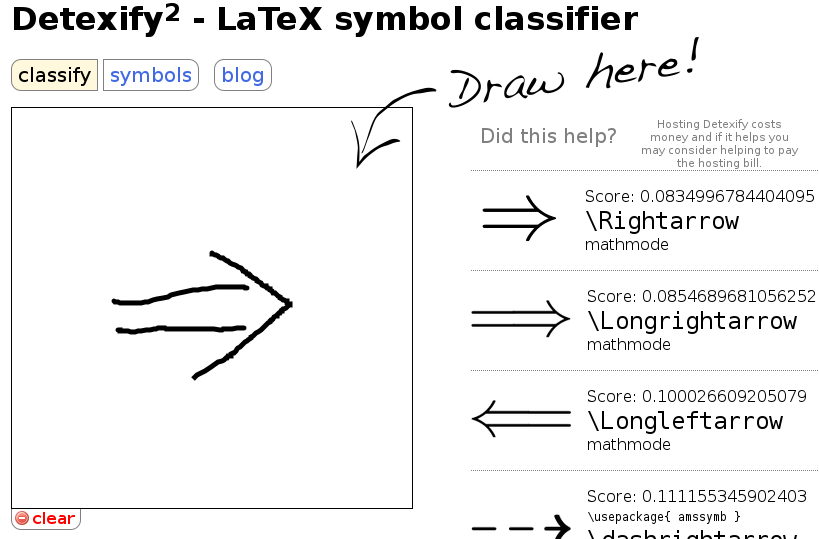
\includegraphics[height=0.48\textheight]{images/detexify}
			\vspace{0.5cm}
			\Large \href{http://detexify.kirelabs.org/}{detexify.kirelabs.org}
			\end{center}
		\end{minipage}
		\begin{minipage}{0.45\textwidth}
			\begin{center}
			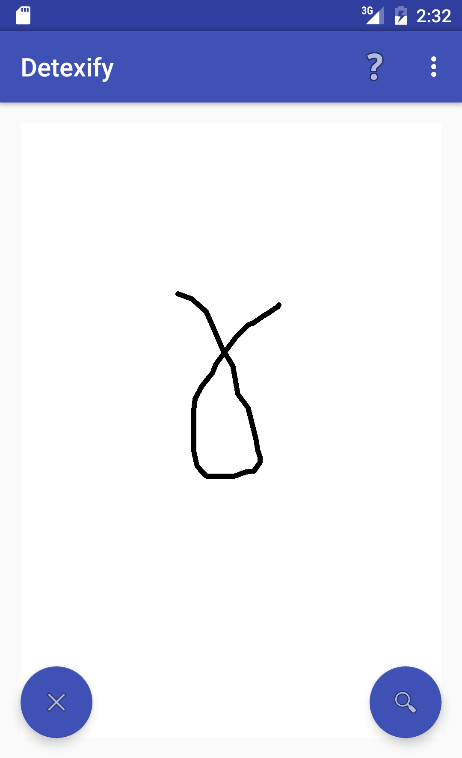
\includegraphics[height=0.48\textheight]{images/detexify-app1}
			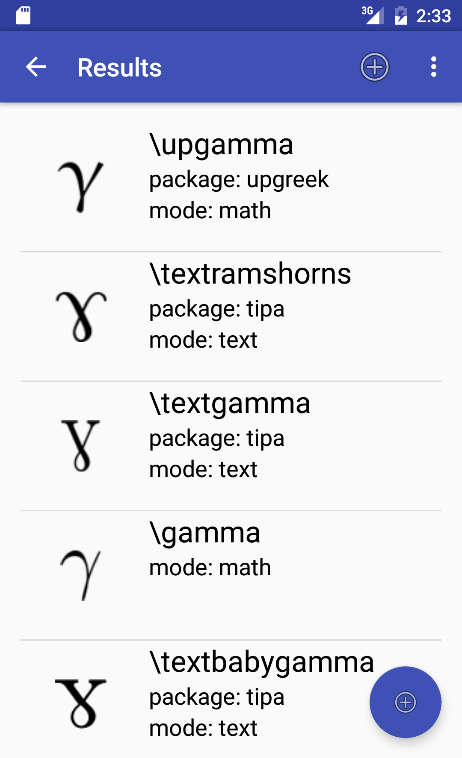
\includegraphics[height=0.48\textheight]{images/detexify-app2}
			\vspace{0.5cm}
			\Large \href{https://play.google.com/store/apps/details?id=website.marty.detexify}{Detexify im Play Store}
			\end{center}
		\end{minipage}
				
		\end{frame}

		
		%%%%%%%%%%%%%%%%%%%%%%%%%%%%%%%%%%%%%%%%%%%%%%%%%%%%%%%%%%%%%%%%%%%%%%%
		
		\begin{frame}{Anmerkungen}
			\slideheading{Achtung:} \TeX{} ist eine Programmiersprache! Lasst nur vertrauenswürdige
			Menschen \TeX/\LaTeX-Code auf eurem Rechner/Server ausführen.
			
			\vspace{0.2cm}
			\slideheading{Anmerkung:} Man kann \textbf{\url{https://www.overleaf.com}} zum live-nachcoden benutzen.
		\end{frame}
		
		%%%%%%%%%%%%%%%%%%%%%%%%%%%%%%%%%%%%%%%%%%%%%%%%%%%%%%%%%%%%%%%%%%%%%%%
		
		\section{Grundlagen von \LaTeX{} und \TeX}
		\subsection{Theorie}
		
		\begin{frame}{Dokumentenklassen}
			\begin{itemize}
				\item Die Dokumentenklasse beschreibt wie ein Dokument aussieht
				\item Ihr beschreibt was ihr schreibt (z.\,B. was eine Überschrift ist)
				\item \LaTeX{} formatiert euer Dokument mit Hilfe der Dokumentenklasse, \textbf{nicht ihr}!
			\end{itemize}
			\vspace{0.1cm}
			\slideheading{Beispiele für Dokumentenklassen:}
			\begin{description}
				\item[scrartcl, article:] Artikel im Umfang von mehreren Seiten
				\item[scrlttr2, letter:] Briefe
				\item[scrreprt, report:] Reports, Umfang mehr als 15 Seiten
				\item[scrbook, book:] Bücher
			\end{description}
		\end{frame}
		
		%%%%%%%%%%%%%%%%%%%%%%%%%%%%%%%%%%%%%%%%%%%%%%%%%%%%%%%%%%%%%%%%%%%%%%%
		
		\begin{frame}{Syntax - Befehle und Umgebungen}
			\slideheading{Befehle:}
			\begin{itemize}
				\item Beginnen mit einem Backslash ( \textbackslash... )
				\item Parameter in geschweiften Klammern ( \{...\} )
				\item \textit{Optionale} Parameter in eckigen ( [...] )
				\item Manchmal auch als \texttt{*}-Variante (leicht verändertes Verhalten; s. \texttt{align} und \texttt{align*} Umgebung später)
			\end{itemize}
			\slideheading{Umgebungen:}
			\begin{itemize}
				\item Beginnen mit dem \texttt{\textbackslash begin\{name\}} Befehl
				\item und enden mit dem \texttt{\textbackslash end\{name\}} Befehl
				\item Formatieren ganze Textblöcke
			\end{itemize}
		\end{frame}
		
		%%%%%%%%%%%%%%%%%%%%%%%%%%%%%%%%%%%%%%%%%%%%%%%%%%%%%%%%%%%%%%%%%%%%%%%
		
		\begin{frame}{Aufbau des Dokumentes}
			\slideheading{Dokument:}
			\begin{enumerate}
				\item Dokumentenklasse wählen
				\item Pakete laden
				\item Einstellungen vornehmen, Styles ändern, Befehle definieren, et.
				\item Dokument öffnen
				\item Inhalte schreiben
				\item Dokument schließen
			\end{enumerate}
		\end{frame}
		
		%%%%%%%%%%%%%%%%%%%%%%%%%%%%%%%%%%%%%%%%%%%%%%%%%%%%%%%%%%%%%%%%%%%%%%%
		
		\begin{frame}{Schriftgrößen}
			\slideheading{Schriftgrößen:}\hspace{5mm}
			\begin{tabular}{l l}
				tiny 			& \tiny\textbackslash tiny\normalsize\\
				scriptsize 		& \scriptsize\textbackslash scriptsize\normalsize\\
				footnotesize 	& \footnotesize\textbackslash footnotesize\normalsize\\
				small 			& \small\textbackslash small\normalsize\\
				normalsize 		& \normalsize\textbackslash normalsize\normalsize\\
				large 			& \large\textbackslash large\normalsize\\
				Large 			& \Large\textbackslash Large\normalsize\\
				LARGE 			& \LARGE\textbackslash LARGE\normalsize\\
				huge 			& \huge\textbackslash huge\normalsize\\
				Huge 			& \Huge\textbackslash Huge\normalsize
			\end{tabular}
		\end{frame}
		
		%%%%%%%%%%%%%%%%%%%%%%%%%%%%%%%%%%%%%%%%%%%%%%%%%%%%%%%%%%%%%%%%%%%%%%%
		
		\subsection{Textsatz-Grundlagen}
		
		\begin{frame}[containsverbatim]{Mein erstes Dokument}
			\begin{latexcode}
\documentclass[a4paper,10pt]{scrartcl}
\usepackage[utf8]{inputenc}
\usepackage[T1]{fontenc}
\usepackage[ngerman]{babel}
\usepackage{lmodern}

\author{Max Mustermann}
\title{Mein erstes Dokument}

\begin{document}
	\maketitle
	Hello World!
\end{document}
			\end{latexcode}
			\begin{textblock}{10}(7.5,10.5)
				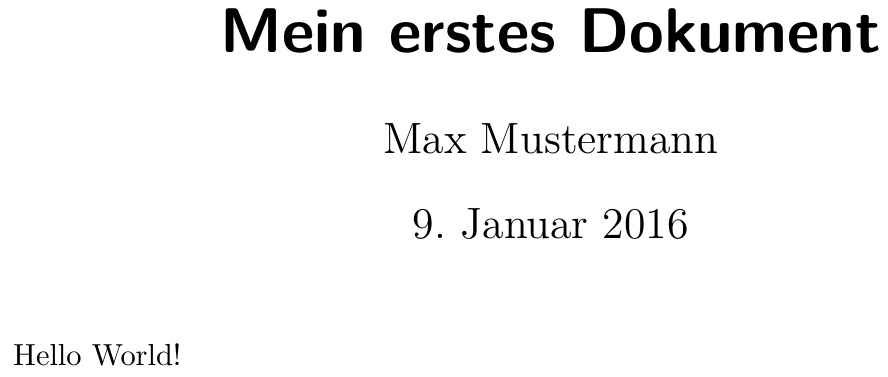
\includegraphics[width=5.5cm]{images/erstes-dokument-scrartcl}
			\end{textblock}
		\end{frame}
		
		%%%%%%%%%%%%%%%%%%%%%%%%%%%%%%%%%%%%%%%%%%%%%%%%%%%%%%%%%%%%%%%%%%%%%%%
		
		\begin{frame}[containsverbatim]{Mein erstes Dokument}
			\begin{latexcode}
\documentclass[a4paper,10pt]{article}
\usepackage[utf8]{inputenc}
\usepackage[T1]{fontenc}
\usepackage[ngerman]{babel}
\usepackage{lmodern}

\author{Max Mustermann}
\title{Mein erstes Dokument}

\begin{document}
	\maketitle
	Hello World!
\end{document}
			\end{latexcode}
			\begin{textblock}{10}(7.5,10.5)
				
\includegraphics[width=5.5cm]{images/erstes-dokument-article}
			\end{textblock}
		\end{frame}
		
		%%%%%%%%%%%%%%%%%%%%%%%%%%%%%%%%%%%%%%%%%%%%%%%%%%%%%%%%%%%%%%%%%%%%%%%
		
		\begin{frame}[containsverbatim]{Gliederung des Dokumentes}
			\slideheading{\LaTeX-Code:}
			\begin{latexcode}
\section{Finden von maximalen Cliquen in Graphen}
Maximale Cliquen haben viele reale Anwendungsfälle.
\subsection{NP-Vollständigkeit}
Das Problem ist NP-vollständig.
			\end{latexcode}
			
			\vspace{0.1cm}
			\slideheading{Ergebnis:}
			\vspace{0.3cm}\\
			{\Large \textbf{1 Finden von maximalen Cliquen}}
			\vspace{2mm}\\
			Maximale Cliquen haben viele reale Anwendungsfälle.
			\vspace{4mm}\\
			\textbf{1.1 NP-Vollständigkeit}
			\vspace{2mm}\\
			Das Problem ist NP-vollständig.
		\end{frame}
		
		%%%%%%%%%%%%%%%%%%%%%%%%%%%%%%%%%%%%%%%%%%%%%%%%%%%%%%%%%%%%%%%%%%%%%%%
		
		\begin{frame}[containsverbatim]{Einfache Textformatierung}
			\begin{columns}[t]
				\column{.5\textwidth}
				\slideheading{\LaTeX-Code:}
				\begin{latexcode}
Dieser Text hat einen\\
Zeilenumbruch.
Dieser       Text\newline
auch

Dies ist ein Absatz
				\end{latexcode}
				\column{.5\textwidth}
				\slideheading{Ergebnis:}
				\vspace{1mm}\\
				Dieser Text hat einen\\
				Zeilenumbruch
				Dieser       Text\newline
				auch
				
				~~~~Dies ist ein Absatz
			\end{columns}
		\end{frame}
		
		%%%%%%%%%%%%%%%%%%%%%%%%%%%%%%%%%%%%%%%%%%%%%%%%%%%%%%%%%%%%%%%%%%%%%%%
		
		\begin{frame}[containsverbatim]{Einfache Textformatierung}
			\slideheading{\LaTeX-Code:}
			\begin{latexcode}
Dies ist \textbf{fett} oder \texttt{typewriter}
oder \textit{kursiv}. Oder einfach nur
\emph{hervorgehoben}.
			\end{latexcode}
			
			\vspace{0.1cm}
			\slideheading{Ergebnis:}
			\vspace{0.1cm}\\
			Dies ist \textbf{fett} oder \texttt{typewriter} oder
			\textit{kursiv}. Oder einfach nur \emph{hervorgehoben}.
		\end{frame}
		
		%%%%%%%%%%%%%%%%%%%%%%%%%%%%%%%%%%%%%%%%%%%%%%%%%%%%%%%%%%%%%%%%%%%%%%%
		
		\begin{frame}[containsverbatim]{(Nummerierte) Auflistungen}
			\begin{columns}
				\column{.5\textwidth}
				\slideheading{\LaTeX-Code:}
				\begin{latexcode}
\begin{itemize}
	\item Kartoffeln
	\item Butter
	\item Milch
\end{itemize}
				\end{latexcode}
				
				\slideheading{Ergebnis:}
				\begin{itemize}
					\item Kartoffeln
					\item Butter
					\item Milch
				\end{itemize}
				 
				\column{.5\textwidth}
				\slideheading{\LaTeX-Code:}
				\begin{latexcode}
\begin{enumerate}
	\item Kartoffeln
	\item Butter
	\item Milch
\end{enumerate}
				\end{latexcode}
				
				\slideheading{Ergebnis:}
				\begin{enumerate}
					\item Kartoffeln
					\item Butter
					\item Milch
				\end{enumerate}
			\end{columns}
		\end{frame}
	
		%%%%%%%%%%%%%%%%%%%%%%%%%%%%%%%%%%%%%%%%%%%%%%%%%%%%%%%%%%%%%%%%%%%%%%%
		
		\begin{frame}[t]{Übung}
			\slideheading{Übung:}
			\vspace{0.1cm}\\
			Schachtel eine Aufzählung, so wie hier:\vspace{0.2cm}\\
			\begin{itemize}
				\item Kartoffeln
				\begin{itemize}
					\item Festkochend
					\item Mehligkochend
				\end{itemize}
				\item Butter
				\item Milch
			\end{itemize}
		\end{frame}
		
		%%%%%%%%%%%%%%%%%%%%%%%%%%%%%%%%%%%%%%%%%%%%%%%%%%%%%%%%%%%%%%%%%%%%%%%
		
		\begin{frame}[t,containsverbatim]{Geschachtelte Auflistungen}
			\begin{columns}[t]
				\column{.6\textwidth}
				\slideheading{\LaTeX-Code:}
				\begin{latexcode}
\begin{itemize}
	\item Kartoffeln
	\begin{itemize}
		\item Festkochend
		\item Mehligkochend
	\end{itemize}
	\item Butter
	\item Milch
\end{itemize}
				\end{latexcode}
				\column{.4\textwidth}
				\slideheading{Ergebnis:}
				\begin{itemize}
					\item Kartoffeln
					\begin{itemize}
						\item Festkochend
						\item Mehligkochend
					\end{itemize}
					\item Butter
					\item Milch
				\end{itemize}
			\end{columns}
		\end{frame}
		
		%%%%%%%%%%%%%%%%%%%%%%%%%%%%%%%%%%%%%%%%%%%%%%%%%%%%%%%%%%%%%%%%%%%%%%%
		
		\begin{frame}[containsverbatim]{\texttt{enumerate}-Packet}
			\begin{columns}[t]
				\column{.6\textwidth}
				\slideheading{\LaTeX-Code:}
				\begin{latexcode}
\usepackage{enumerate}
% ...
\begin{enumerate}[I.]
	\item Erster Punkt
	    \begin{enumerate}[A]
	    \item Erster Unterpunkt
	    \item Zweiter Unterpunkte
	    \end{enumerate}
	\item Zweiter Punkt
	\item Dritter Punkt
\end{enumerate}
				\end{latexcode}
				
				\column{.4\textwidth}
				\slideheading{Ergebnis:}
				\begin{enumerate}[I.]
					\item Erster Punkt
					    \begin{enumerate}[A]
					    \item Erster Unterpunkt
					    \item Zweiter Unterpunkte
					    \end{enumerate}
					\item Zweiter Punkt
					\item Dritter Punkt
				\end{enumerate}
			\end{columns}
		\end{frame}
		
		%%%%%%%%%%%%%%%%%%%%%%%%%%%%%%%%%%%%%%%%%%%%%%%%%%%%%%%%%%%%%%%%%%%%%%%
		
		\begin{frame}[containsverbatim]{\texttt{enumerate}-Packet}
			\begin{columns}[t]
				\column{.6\textwidth}
				\slideheading{\LaTeX-Code:}
				\begin{latexcode}
\usepackage{enumerate}
% ...
\begin{enumerate}[1]
	\item Erster Punkt
	    \begin{enumerate}[(a).]
	    \item Erster Unterpunkt
	    \item Zweiter Unterpunkte
	    \end{enumerate}
	\item Zweiter Punkt
	\item Dritter Punkt
\end{enumerate}
				\end{latexcode}
				
				\column{.4\textwidth}
				\slideheading{Ergebnis:}
				\begin{enumerate}[1]
					\item Erster Punkt
					    \begin{enumerate}[(a).]
					    \item Erster Unterpunkt
					    \item Zweiter Unterpunkte
					    \end{enumerate}
					\item Zweiter Punkt
					\item Dritter Punkt
				\end{enumerate}
			\end{columns}
		\end{frame}
		
		%%%%%%%%%%%%%%%%%%%%%%%%%%%%%%%%%%%%%%%%%%%%%%%%%%%%%%%%%%%%%%%%%%%%%%%
		
		\begin{frame}[containsverbatim]{Definitionslisten}
			\slideheading{\LaTeX-Code:}
			\begin{latexcode}
\begin{description}
	\item[Kile] Guter Editor für GNU/Linux (KDE).
	\item[AUCTeX] für Emacs-Benutzer
	\item[Texmaker] Editor für alle Betriebssysteme
\end{description}
			\end{latexcode}
			
			\slideheading{Ergebnis:}
			\begin{description}
				\item[Kile] Einfacher Editor für GNU/Linux (KDE).
				\item[AUCTeX] für Emacs-Benutzer
				\item[Texmaker] Editor für alle Betriebssysteme
			\end{description}
		\end{frame}
		
		%%%%%%%%%%%%%%%%%%%%%%%%%%%%%%%%%%%%%%%%%%%%%%%%%%%%%%%%%%%%%%%%%%%%%%%
		
		\begin{frame}[containsverbatim]{Tabellen}
			\begin{columns}[t]
				\column{0.55\textwidth}
				\slideheading{\LaTeX-Code:}
				\begin{latexcode}
\begin{tabular}{l||c|r}
	Händler & Produkt & Preis\\
	\hline
	\hline
	Ohbi & Fliesen & 17,95\\
	Porsche & Motor & 270,15\\
	\hline
	Farber & Stift & 2,99
\end{tabular}
				\end{latexcode}
				
				\column{0.45\textwidth}
				\slideheading{Ergebnis:}
				\vspace{0.1cm}\\
				\begin{tabular}{l||c|r}
					Händler & Produkt & Preis\\
					\hline
					\hline
					Ohbi & Fliesen & 17,95\\
					Porsche & Motor & 270,15\\
					\hline
					Farber & Stift & 2,99
				\end{tabular}
			\end{columns}
		\end{frame}
			
		%%%%%%%%%%%%%%%%%%%%%%%%%%%%%%%%%%%%%%%%%%%%%%%%%%%%%%%%%%%%%%%%%%%%%%%
		
		\begin{frame}[t]{Übung}
			\slideheading{Übung:}
			\vspace{0.1cm}\\
			Erstelle eine Tabelle mit \textbf{automatischem} Zeilenumbruch:\vspace{0.2cm}\\
			
			\begin{tabular}{l|p{7cm}}
				Spalte 1 & Spalte 2 \\ \hline
				Foo & Lorem ipsum dolor sit amet, consectetur adipiscing elit. \\
				Bar & Lorem ipsum [...]
			\end{tabular}
		\end{frame}
		
		%%%%%%%%%%%%%%%%%%%%%%%%%%%%%%%%%%%%%%%%%%%%%%%%%%%%%%%%%%%%%%%%%%%%%%%
		
%		\begin{frame}[containsverbatim]{Tabellen mit \texttt{longtable}}
		\begin{frame}[containsverbatim]{Spaltentyp \texttt{p\{<breite>\}}}
			\slideheading{\LaTeX-Code:}
			\begin{latexcode}
\begin{tabular}{l|p{8cm}}
Spalte 1 & Spalte 2 \\ \hline
Foo & Lorem ipsum dolor sit amet [...] \\
Bar & Lorem ipsum [...]
\end{tabular}
			\end{latexcode}
			
			\slideheading{Ergebnis:}
			\vspace{0.1cm}\\
			\begin{tabular}{l|p{7cm}}
				Spalte 1 & Spalte 2 \\ \hline
				Foo & Lorem ipsum dolor sit amet, consectetur adipiscing elit. \\
				Bar & Lorem ipsum [...]
			\end{tabular}
		\end{frame}
		
		\begin{frame}[containsverbatim]{Automatische Breite mit \texttt{tabularx}}
			\slideheading{\LaTeX-Code:}
			\begin{latexcode}
\begin{tabularx}{.85\textwidth}{l|X}
Spalte 1 & Spalte 2 \\ \hline
Foo & Lorem ipsum dolor sit amet [...] \\
Bar & Lorem ipsum [...]
\end{tabularx}
			\end{latexcode}
			
			\slideheading{Ergebnis:}
			\vspace{0.1cm}\\
			\begin{tabularx}{.85\textwidth}{l|X}
				Spalte 1 & Spalte 2 \\ \hline
				Foo & Lorem ipsum dolor sit amet, consectetur adipiscing elit. \\
				Bar & Lorem ipsum [...]
			\end{tabularx}
		\end{frame}
		
		%%%%%%%%%%%%%%%%%%%%%%%%%%%%%%%%%%%%%%%%%%%%%%%%%%%%%%%%%%%%%%%%%%%%%%%
		
		\begin{frame}[containsverbatim]{Grafiken einbinden}
			\slideheading{\LaTeX-Code:}
			\begin{latexcode}
\usepackage{graphicx}

\includegraphics[width=3cm]{images/gnu}
			\end{latexcode}
			
			\slideheading{Ergebnis:}
			
\includegraphics[width=2.5cm]{images/gnu}
		\end{frame}
		
		%%%%%%%%%%%%%%%%%%%%%%%%%%%%%%%%%%%%%%%%%%%%%%%%%%%%%%%%%%%%%%%%%%%%%%%
		
		\begin{frame}[containsverbatim]{\texttt{ams}-Pakete der American Mathematical Society}
			Für komplexere mathematische Darstellungen müssen die
			\texttt{ams}-Pakete der American Mathematical Society eingebunden
			werden.
			
			\vspace{0.5cm}
			\slideheading{\LaTeX{}-Code:}
			\begin{latexcode}
% Im Header
\usepackage{amsmath}
\usepackage{amsfonts}
\usepackage{amssymb}
			\end{latexcode}
		\end{frame}
		
		%%%%%%%%%%%%%%%%%%%%%%%%%%%%%%%%%%%%%%%%%%%%%%%%%%%%%%%%%%%%%%%%%%%%%%%
		
	\section{Mathematischer Textsatz}
		\subsection{Theorie}
		\begin{frame}[containsverbatim]{Mathe-Umgebung}
			Es gibt verschiedene Mathe-Umgebungen:
			\begin{itemize}
				\item Die \texttt{\$...\$} Umgebung
				\begin{itemize}
					\item Mathe innerhalb von Text (stammt nicht aus \LaTeX, sondern aus \TeX{} und sollte vermieden werden)
				\end{itemize}
				\item Die \texttt{\textbackslash(...\textbackslash)} Umgebung
				\begin{itemize}
					\item Mathe innerhalb von Text (stammt aus \LaTeX und funktioniert besser mit den \texttt{ams}-Paketen)
				\end{itemize}
				\item Die \texttt{\textbackslash[...\textbackslash]} Umgebung
				\begin{itemize}
					\item Einzeilige Matheumgebung für eine Formel/Gleichung
				\end{itemize}
			\end{itemize}
		\end{frame}
		
		%%%%%%%%%%%%%%%%%%%%%%%%%%%%%%%%%%%%%%%%%%%%%%%%%%%%%%%%%%%%%%%%%%%%%%%
		
		\begin{frame}[containsverbatim]{Mathe-Umgebung}
			\slideheading{\LaTeX{}-Code:}
			\begin{latexcode}
Wir können im Text Wurzeln, wie z.\,B. \( \sqrt{2} \)
verwenden. Oder auch Matheformeln als ganzen Block:
\[ \sum_{k=1}^n k = \frac{n(n+1)}{2} \]
			\end{latexcode}
			
			\slideheading{Ergebnis:}
			Wir können im Text Wurzeln, wie z.\,B. \( \sqrt{2} \)
			verwenden. Oder auch Matheformeln als ganzen Block:
			\[ \sum_{k=1}^n k = \frac{n(n+1)}{2} \]
		\end{frame}
		
		%%%%%%%%%%%%%%%%%%%%%%%%%%%%%%%%%%%%%%%%%%%%%%%%%%%%%%%%%%%%%%%%%%%%%%%
		
		\begin{frame}[containsverbatim]{Mathe-Umgebung}
			\slideheading{\LaTeX{}-Code:}
			\begin{latexcode}
Neben Summen ($\sum$) gibt es auch Integrale:
\[ \int\limits_a^b f(x) \ \mathrm{d}x \]
			\end{latexcode}
			
			\slideheading{Ergebnis:}
			Neben Summen ($\sum$) gibt es auch Integrale:
			\[ \int\limits_a^b f(x) \ \mathrm{d}x \]
		\end{frame}
		
		%%%%%%%%%%%%%%%%%%%%%%%%%%%%%%%%%%%%%%%%%%%%%%%%%%%%%%%%%%%%%%%%%%%%%%%
		
		\begin{frame}[containsverbatim]{Mathe-Umgebung}
			\slideheading{\LaTeX{}-Code:}
			\begin{latexcode}
Die Probleminstanz \(\mathfrak{B}\) sei gegeben Durch
die Menge \(\mathbb{N}\) und einer Zahl \(n\), sowie
der Eingabe \(\mathcal{A}\).
			\end{latexcode}
			
			\slideheading{Ergebnis:}
Die Probleminstanz \(\mathfrak{B}\) sei gegeben Durch die Menge \(\mathbb{N}\) und einer Zahl \(n\), sowie der Eingabe \(\mathcal{A}\).
		\end{frame}
		
		%%%%%%%%%%%%%%%%%%%%%%%%%%%%%%%%%%%%%%%%%%%%%%%%%%%%%%%%%%%%%%%%%%%%%%%
		
		\begin{frame}[containsverbatim]{Mathebeispiele: Matrizen}
			\slideheading{\LaTeX{}-Code:}
			\begin{latexcode}
\begin{pmatrix}
	\cos(\alpha)  & \sin(\alpha) & 0 & 0 \\
	-\sin(\alpha) & \cos(\alpha) & 0 & 0 \\
	            0 &            0 & 1 & 0 \\
	            0 &            0 & 0 & 1
\end{pmatrix}
			\end{latexcode}
			
			\slideheading{Ergebnis:}
			\[
				\begin{pmatrix}
				\cos(\alpha)  & \sin(\alpha) & 0 & 0 \\
				-\sin(\alpha) & \cos(\alpha) & 0 & 0 \\
				            0 &            0 & 1 & 0 \\
				            0 &            0 & 0 & 1
				\end{pmatrix}
			\]
		\end{frame}
		
		%%%%%%%%%%%%%%%%%%%%%%%%%%%%%%%%%%%%%%%%%%%%%%%%%%%%%%%%%%%%%%%%%%%%%%%
		
		\subsection{Beispiele}
		\begin{frame}[containsverbatim]{Mathebeispiele: Matrizen}
			\slideheading{\LaTeX{}-Code:}
			\begin{latexcode}
\begin{bmatrix}
	\cos(\alpha)  & \sin(\alpha) & 0 & 0 \\
	-\sin(\alpha) & \cos(\alpha) & 0 & 0 \\
	            0 &            0 & 1 & 0 \\
	            0 &            0 & 0 & 1
\end{bmatrix}
			\end{latexcode}
			
			\slideheading{Ergebnis:}
			\[
				\begin{bmatrix}
				\cos(\alpha)  & \sin(\alpha) & 0 & 0 \\
				-\sin(\alpha) & \cos(\alpha) & 0 & 0 \\
				            0 &            0 & 1 & 0 \\
				            0 &            0 & 0 & 1
				\end{bmatrix}
			\]
		\end{frame}
		
		%%%%%%%%%%%%%%%%%%%%%%%%%%%%%%%%%%%%%%%%%%%%%%%%%%%%%%%%%%%%%%%%%%%%%%%
		
		\begin{frame}[containsverbatim]{Mathebeispiele: Matrizen}
			\slideheading{\LaTeX{}-Code:}
			\begin{latexcode}
\begin{Bmatrix}
	\cos(\alpha)  & \sin(\alpha) & 0 & 0 \\
	-\sin(\alpha) & \cos(\alpha) & 0 & 0 \\
	            0 &            0 & 1 & 0 \\
	            0 &            0 & 0 & 1
\end{Bmatrix}
			\end{latexcode}
			
			\slideheading{Ergebnis:}
			\[
				\begin{Bmatrix}
				\cos(\alpha)  & \sin(\alpha) & 0 & 0 \\
				-\sin(\alpha) & \cos(\alpha) & 0 & 0 \\
				            0 &            0 & 1 & 0 \\
				            0 &            0 & 0 & 1
				\end{Bmatrix}
			\]
		\end{frame}
		
		%%%%%%%%%%%%%%%%%%%%%%%%%%%%%%%%%%%%%%%%%%%%%%%%%%%%%%%%%%%%%%%%%%%%%%%
		
		\begin{frame}[containsverbatim]{Mathebeispiele: Gleichungssysteme}
			\slideheading{\LaTeX{}-Code:}
			\begin{latexcode}
\begin{align}
	\sin^2(\alpha) + \cos^2(\alpha) & = 1 \\
	\tan(\alpha) & = \frac{\sin(\alpha)}{\cos(\alpha)}
\end{align}
			\end{latexcode}
			
			\slideheading{Ergebnis:}
			\begin{align}
				\sin^2(\alpha) + \cos^2(\alpha) & = 1 \\
				\tan(\alpha) & = \frac{\sin(\alpha)}{\cos(\alpha)}
			\end{align}
			\slideheading{Achtung}: \texttt{align} macht automatisch eine Mathe-Umgebung auf!
		\end{frame}
		
		%%%%%%%%%%%%%%%%%%%%%%%%%%%%%%%%%%%%%%%%%%%%%%%%%%%%%%%%%%%%%%%%%%%%%%%
		
		\begin{frame}[containsverbatim]{Mathebeispiele: Gleichungssysteme}
			\slideheading{\LaTeX{}-Code:}
			\begin{latexcode}
\begin{align*}
	\sin^2(\alpha) + \cos^2(\alpha) & = 1 \\
	\tan(\alpha) & = \frac{\sin(\alpha)}{\cos(\alpha)}
\end{align*}
			\end{latexcode}
			
			\slideheading{Ergebnis:}
			\begin{align*}
				\sin^2(\alpha) + \cos^2(\alpha) & = 1 \\
				\tan(\alpha) & = \frac{\sin(\alpha)}{\cos(\alpha)}
			\end{align*}
			\slideheading{Achtung}: \texttt{align} macht automatisch eine Mathe-Umgebung auf!
		\end{frame}
		
		%%%%%%%%%%%%%%%%%%%%%%%%%%%%%%%%%%%%%%%%%%%%%%%%%%%%%%%%%%%%%%%%%%%%%%%
		
		\begin{frame}[containsverbatim]{Mathebeispiele: Fallunterscheidung}
		
		\slideheading{\LaTeX{}-Code:}
		\begin{latexcode}
 fib(n) =
 \begin{cases}
	 0                   & \text{wenn } n = 0 \\
	 1                   & \text{wenn } n = 1 \\
	 fib(n-1) + fib(n-2) & \text{sonst}
 \end{cases}
		\end{latexcode}
		  
		\slideheading{Ergebnis:}
		\[
		  fib(n) =
		 \begin{cases}
			 0                   & \text{wenn } n = 0 \\
			 1                   & \text{wenn } n = 1 \\
			 fib(n-1) + fib(n-2) & \text{sonst}
		 \end{cases}
		\]
		\end{frame}
	
		%%%%%%%%%%%%%%%%%%%%%%%%%%%%%%%%%%%%%%%%%%%%%%%%%%%%%%%%%%%%%%%%%%%%%%%
		
		\begin{frame}[t]{Finale Übung}
			\slideheading{Übung:} Bilde dieses Dokument nach:\vspace{0.2cm}
			
			\begin{center}
				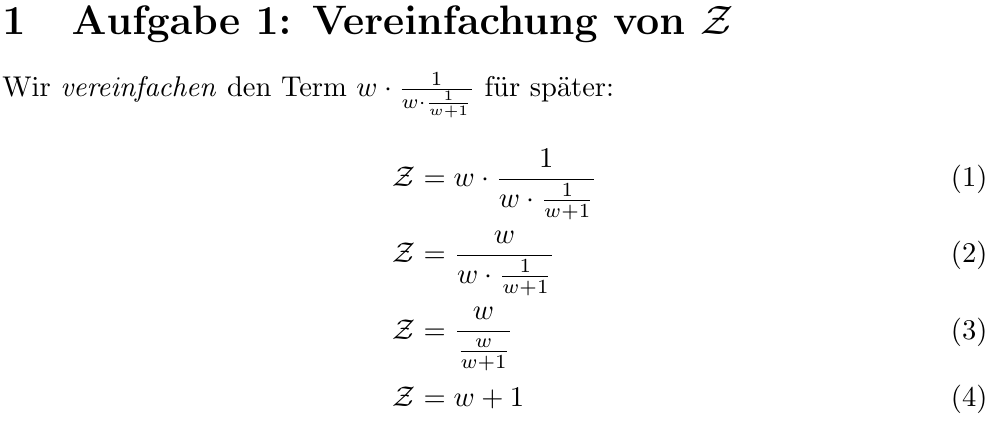
\includegraphics[width=0.95\textwidth]{images/mathe-uebung-1}
			\end{center}
		\end{frame}
			
		%%%%%%%%%%%%%%%%%%%%%%%%%%%%%%%%%%%%%%%%%%%%%%%%%%%%%%%%%%%%%%%%%%%%%%%
		
		\begin{frame}[containsverbatim]{Finale Übung}
			\slideheading{\LaTeX{}-Code:}\\
			{\footnotesize
			\begin{latexcode}
\section{Aufgabe 1: Vereinfacung von \(\mathcal{Z}\)}
Wir \textit{vereinfachen} den Term
\(w\cdot\frac{1}{w\cdot\frac{1}{w+1}}\) für später:
\begin{align}
	\mathcal{Z} &= w\cdot\frac{1}{w\cdot\frac{1}{w+1}}           \\
	\mathcal{Z} &=       \frac{w}{w\cdot\frac{1}{w+1}}\label{foo}\\
	\mathcal{Z} &=       \frac{w}{      \frac{w}{w+1}}           \\
	\mathcal{Z} &= w+1
\end{align}
Schritt \textbf{\ref{foo}} ist sehr wichtig.
			\end{latexcode}
			}
		\end{frame}
			
		%%%%%%%%%%%%%%%%%%%%%%%%%%%%%%%%%%%%%%%%%%%%%%%%%%%%%%%%%%%%%%%%%%%%%%%
		
	\section*{}
		\begin{frame}
			\begin{center}
				
\includegraphics[height=0.95\textheight]{./images/hotline}
			\end{center}
		\end{frame}
\end{document}